%%%--------------------------------%%%
%%% UC5
%%%--------------------------------%%%

\newpage
% UC5 ====================================================
\subsubsection{Use Case Specification: \ac{UC}5 Risk Pool}
\label{sec:domainBbf}

\paragraph*{Description}\mbox{}\\
The risk pool serves to share knowledge among different teams and to store experiences. Users can vote for project risks to be added to the risk pool. After a certain quorum is reached the risk will be moved to the risk pool and will be persisted together with its responses there. Whenever a new risk is created the user will then have the option to check the pool risks if their risk is already present. They can then add a reference to the pool risks to their project risks. Pool risk can already have responses attached to them and will display the average occurrence probability and impact severity estimates of their project references giving an indication of how other teams evaluated the risk. The individual project risk evaluation process will still be undertaken for pool risks. \\
To remove risks from the risk pool a user will have to request a voting process on the pool risk. They can choose to either have the risk deleted (because it is outdated for example) or to merge it with another risk. All users will then be notified that a pool risk is up for discussion and will be invited to vote. If the vote is favorable the risk will be deleted and in case of a merge request its responses and references will be moved to the merge risk. \\
Quorums can be adjusted by project managers however there will be a notification that the change affects all teams and other project managers will receive a notification should a quorum be changed. 

\paragraph*{Screenshots}\mbox{}\\
Insert screenshots and shortly explain what can be seen
\begin{figure}[h] 
	\centering
	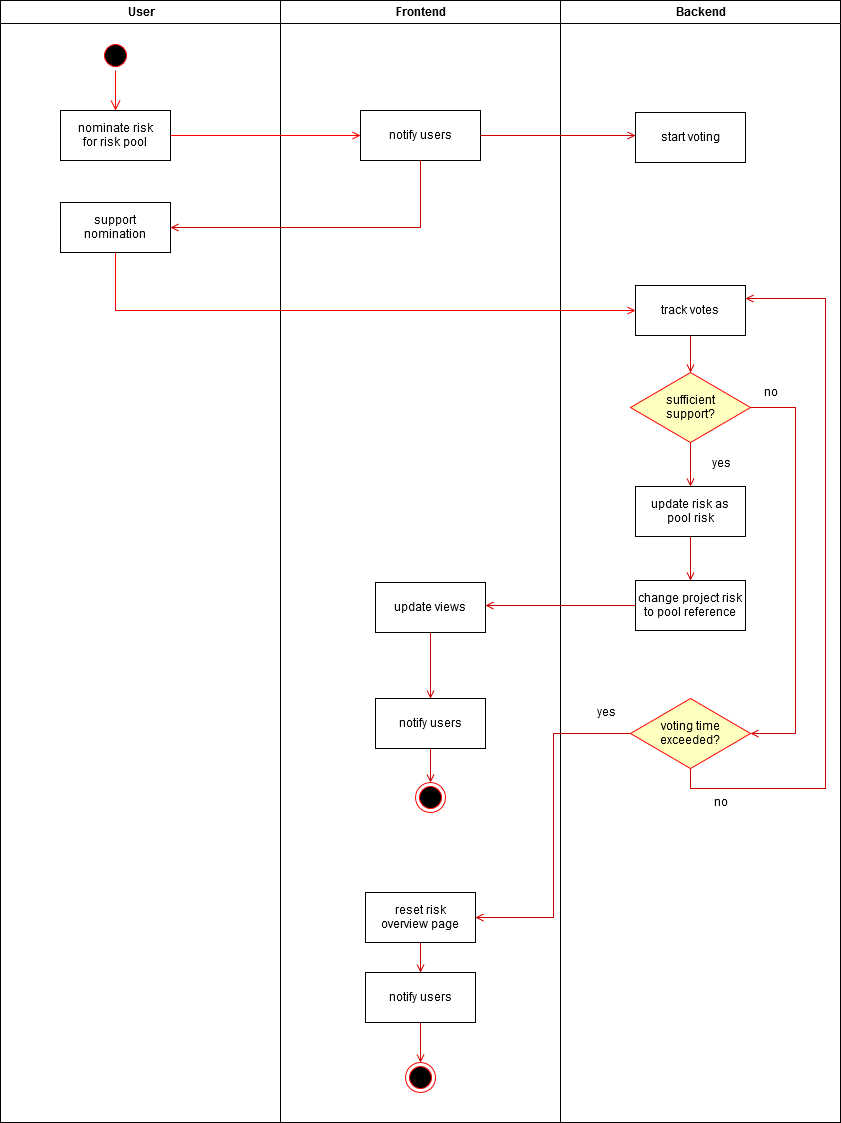
\includegraphics[width=0.8\textwidth]{Content/Domain/UC5RiskPoolDiagram.png}
	\caption{Use Case X: Detail}
	\label{fig:label5}
\end{figure}

\paragraph*{Basic Flow} \mbox{}\\
Add flow:
\begin{itemize}
	\vspace{-3mm}
	\setlength\itemsep{-1em}
	\item A user clicks on the "nominate for risk pool" button on a project risk's detail page.
	\item Other users on the project team will be notified that a risk has been nominated.
	\item The nomination button will be replaced by a support button for these users.
	\item Once a pre-defined quorum of users has supported the nomination the risk will be moved to the risk pool and the project risk will become a reference to the pool risk.
\end{itemize}

Remove flow:
\begin{itemize}
	\vspace{-3mm}
	\setlength\itemsep{-1em}
	\item A user nominates a pool risk for being removed on the pool risk's detail page.
	\item All users who are part of a project that references the pool risks will be notified.
	\item The nomination button will be replaced by a support button for those users.
	\item If a pre-defined quorum of users supports the nomination the project references will be turned into copies of the original risk and the copies risk will be removed from the risk pool.
\end{itemize}

Duplicate flow:
\begin{itemize}
	\vspace{-3mm}
	\setlength\itemsep{-1em}
	\item A user marks a pool risk as being a duplicate.
	\item The user will be shown a list of pool risks to mark the corresponding risk.
	\item All users which are part of projects that reference either risk will be notified.
	\item The nomination button will be replaced by a confirmation button for those users.
	\item If a pre-defined quorum of users confirms the duplication the risks will be merged.
	\item All references of the second risks will be redirected to the first, the response list will be merged and the duplicate will be deleted.
\end{itemize}

\subparagraph{Activity Diagram}\mbox{}\\
\begin{figure}[H]
	\centering
	
\includegraphics[width=0.8\textwidth]{Content/Domain/placeholder.png}
	\caption{Activity Diagram Use Case X}
	\label{fig:label55}
\end{figure}

\paragraph*{Alternative Flows}\mbox{}\\
The last steps of the above described flows will change if the quorum is not met within a pre-defined timeframe.
\begin{itemize}
	\vspace{-3mm}
	\setlength\itemsep{-1em}
	\item The risks will not be changed and the status from before the nomination will be restored.
\end{itemize}

\paragraph*{Special Requirements and Preconditions}\mbox{}\\
This use case has the following preconditions:
\begin{enumerate}
	\vspace{-3mm}
	\setlength\itemsep{-1em}
	\item The user is part of a project which contains risks.
	Or
	\item There is a risk in the risk pool.
	Or
	\item There are two similar risks in the risk pool.
\end{enumerate}

\paragraph*{Postconditions and Persistance}\mbox{}\\
The changes are instantly reflected in the database. Once the changes are confirmed corresponding PUT and DELETE requests update the database.